\section{Inclusive $\pi^{-}$-Argon Cross-Section} \label{sec:CrossSection}
Finally, we come to the inclusive $\pi^{-}$-Argon cross-section result for the data and MC samples defined previously.

The incident kinetic energy is defined as
\begin{equation}
KE_{Incident} = \sqrt{P_{WCtrk}^2 + m_{\pi}^2} - m_{\pi}^2 - E_{Loss} - (\Sigma dE/dX_{i} \times Pitch)
\end{equation}
up to the point of where the track either has an interaction and thus reaches the end of track in the volume or exits out the back. The distribution is shown in Figure \ref{fig:IncidentEnergy}.

\begin{figure}[h!]
\centering
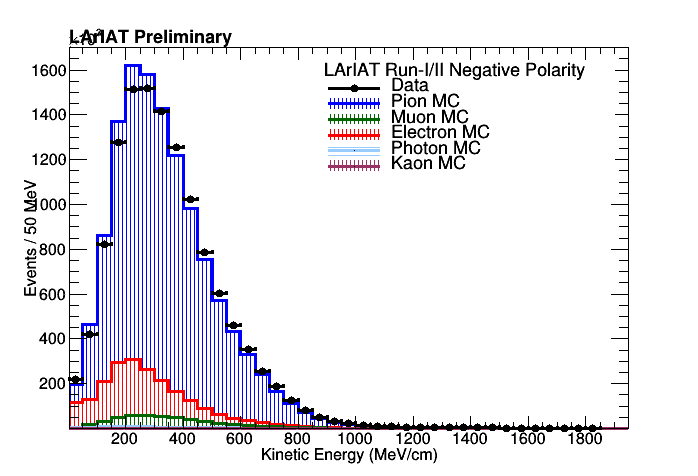
\includegraphics[scale=0.30]{./images/IncidentKE.png}
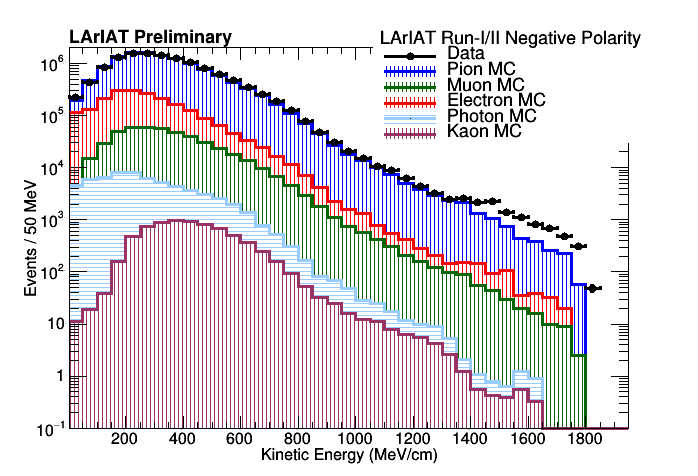
\includegraphics[scale=0.30]{./images/IncidentKELog.png}
\caption{Incident kinetic energy distribution. (Note: the distribution on the left is linear scale in the y-axis, and the distribution on the right is log scale on the y-axis).}
\label{fig:IncidentEnergy}
\end{figure}

Figure \ref{fig:InteractingEnergy} shows the kinetic energy distribution for the interaction point. Tracks which exit out of the active volume of the TPC without having an interaction are excluded from this plot.

\begin{figure}[h!]
\centering
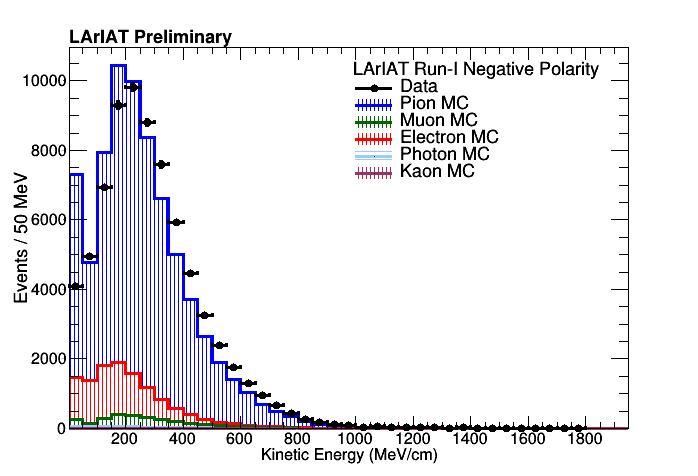
\includegraphics[scale=0.30]{./images/InteractingKE.png}
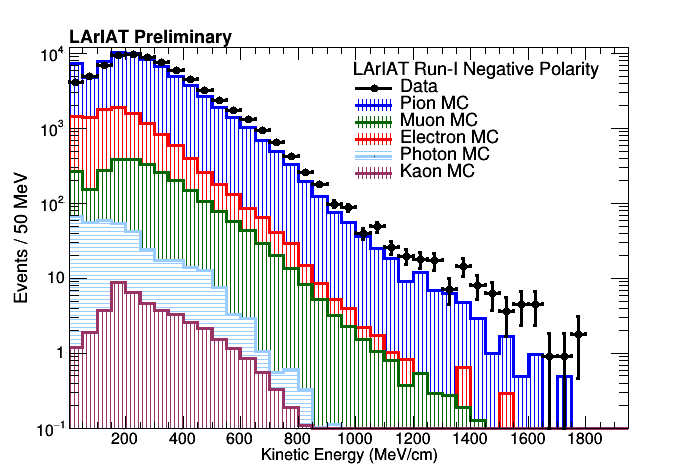
\includegraphics[scale=0.30]{./images/InteractingKELog.png}
\caption{Interacting kinetic energy distribution. (Note: the distribution on the left is linear scale in the y-axis, and the distribution on the right is log scale on the y-axis).}
\label{fig:InteractingEnergy}
\end{figure}

We calculate the cross-section according to the method described in Section \ref{sec:ThinSlice}, correcting for the crossing muon contamination (estimated at 9$\%$), as explained in Appendix \ref{appendix:CrossingMuon}. Figure \ref{fig:RawCrossSection} shows the full range of the computed cross-section including negative kinetic energy bins (between -100 MeV and 0 MeV). There are a few features worth noting about this plot.

\begin{itemize}
\item \textbf{Negative Energy Bins}: The data and the MC don't agree at all in the negative energy bins.

\item \textbf{0~MeV$<$KE$<$50~MeV}: This is the only physical bin in which the data and MC disagree strongly. As outlined in Section \ref{sec:MCReduction}, this bin is expected to be dominated by pion capture-at-rest and should be excluded from the interaction cross-section. This may suggest that the rate at which these events occur is different between data and MC and, while interesting, is beyond the scope of this analysis.

\item \textbf{KE $>$ 50~MeV}: There is generally good agreement above 50~MeV between data and MC.

\end{itemize}

\begin{figure}[h!]
\centering
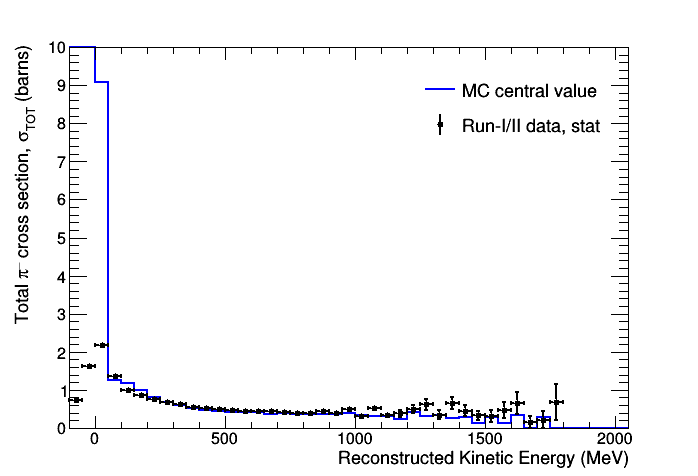
\includegraphics[scale=0.30]{./images/CombinedNegPol_xsec_MC_noband_fineBin.png}
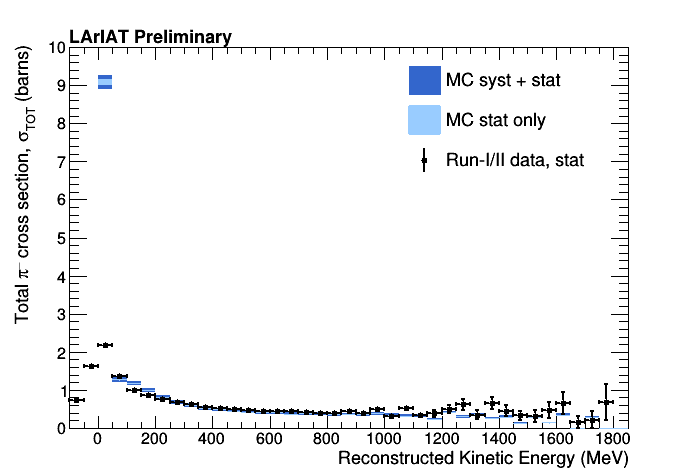
\includegraphics[scale=0.30]{./images/CombinedNegPol_xsec_MCband_opt2FineBin.png}
\caption{Total cross-section computed across the full kinetic energy range (including negative KE bins). The LHS shows the data (black) and the MC central value (blue). The RHS shows the same but with systematic errors associated. }
\label{fig:RawCrossSection}
\end{figure}

Figure \ref{fig:ProperBinCrossSection} shows the inclusive cross-section zoomed in between 50~MeV$<$KE$<$1800 MeV.

\begin{figure}[h!]
\centering
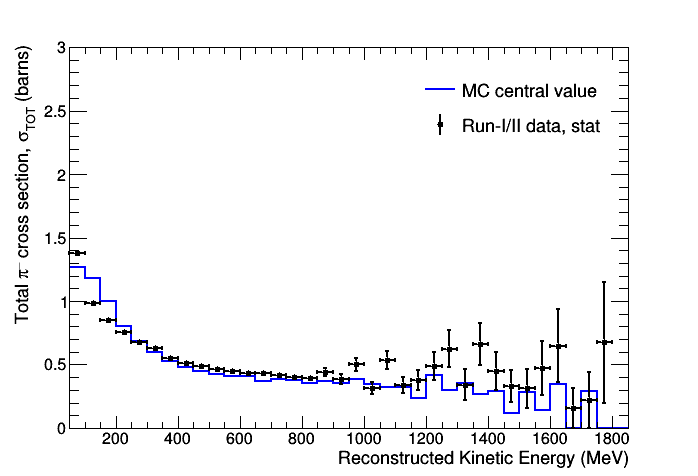
\includegraphics[scale=0.30]{./images/CombinedNegPol_xsec_MC_noband_fineBinProper.png}
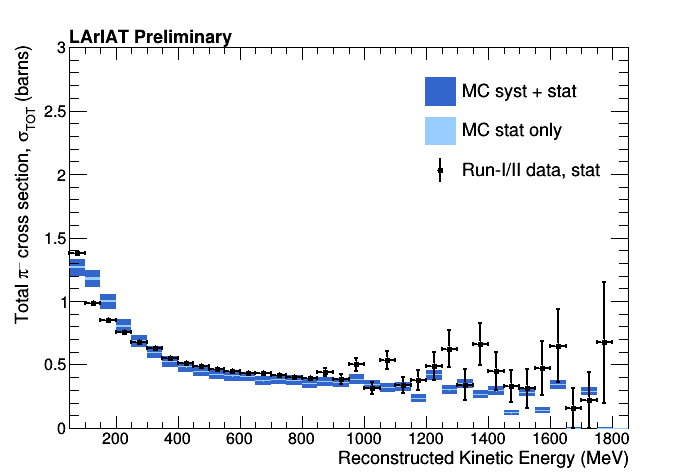
\includegraphics[scale=0.30]{./images/CombinedNegPol_xsec_MCband_opt1FineBinProper.png}
\caption{Total cross-section in the region between 50~MeV$<$KE$<$1800 MeV. The LHS shows the data (black) and the MC central value (blue). The RHS shows the same but with systematic errors associated. }
\label{fig:ProperBinCrossSection}
\end{figure}

Figure \ref{fig:VariableBinCrossSection} shows the final result for the cross-section. In the region between 300~MeV and 1200~MeV the data is 6-8$\%$ higher than the Monte Carlo prediction, but within the systematic uncertainty of the measurement. The region below 300~MeV is data is low compared to the MC (with the exception of the lowest energy bin).


\begin{figure}[h!]
\centering
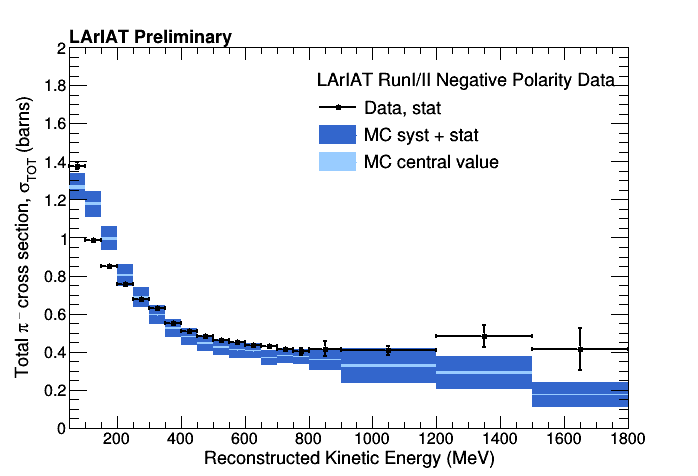
\includegraphics[scale=0.60]{./images/TotalCrossSection.png}
\caption{Total cross-section in the region between 50~MeV$<$KE$<$1800 MeV. }
\label{fig:VariableBinCrossSection}
\end{figure}

\clearpage


\newpage